\documentclass[10pt,a4paper]{article}
\usepackage[margin=2.3cm]{geometry}
\usepackage[T1]{fontenc}
\usepackage{lmodern,microtype,booktabs,graphicx,amsmath,amssymb,xcolor,hyperref,caption,enumitem}
\usepackage[numbers]{natbib}
\hypersetup{colorlinks=true,linkcolor=blue!50!black,citecolor=blue!50!black,urlcolor=blue!50!black}
\captionsetup{font=small,labelfont=bf}
\setlist{nosep}
\newcommand{\tauE}{\tau_e}

\title{Aggregating CausalRivers creates contemporaneous edges, but orientation there is dominated by scale leakage and shared forcing: AUROC gains over lag-only VAR reflect skeleton detection}
\author{Author list to be decided}
\date{Draft, \today}

\begin{document}
\maketitle

\begin{abstract}
Temporal aggregation turns upstream-to-downstream river edges with short travel times into contemporaneous edges whose direction is known from physics. We examine whether this makes aggregated CausalRivers a usable real-data benchmark for contemporaneous causal discovery. We label each edge by its empirical travel time estimated from 15-minute cross-correlation, check three validity gates, and compare lag-only VAR and correlation scores with PCMCI+, VAR-LiNGAM and a DYNOTEARS implementation on 100 held-out subgraphs at 6\,h, 12\,h and 24\,h. The gates pass (pooled), with two caveats: the physics orientation is consistent with the data for only 62.4\% of East German edges, and 6\,h has too few contemporaneous edges. The pre-registered positive hypothesis fails: at 24\,h no method reaches the pre-set accuracy of 0.60 on contemporaneous edges, and at 12\,h only VAR-LiNGAM does (0.611, 95\% CI [0.565, 0.660]). Contemporaneous-capable methods beat lag-only VAR in directed AUROC (by 0.12 to 0.16 at 24\,h for PCMCI+ and DYNOTEARS), but the symmetric $|$correlation$|$ score, which cannot orient anything, reaches 0.684 at 24\,h and matches PCMCI+. A control that regresses each station on all others at the same time step orients 72--74\% of contemporaneous edges correctly, better than every method, and the residual correlation among sibling stations (0.51 at 24\,h) equals that of unrelated pairs. Orientation accuracy on this benchmark therefore cannot be credited to modelling contemporaneous mechanisms. We report the protocol, the gates and the deviations from our pre-registered plan.
\end{abstract}

\section{Introduction}
Methods for time-series causal discovery that model same-step (contemporaneous) effects, such as PCMCI+ \citep{runge2020pcmciplus}, VAR-LiNGAM \citep{hyvarinen2010svar} and DYNOTEARS \citep{pamfil2020dynotears}, are mostly validated on synthetic data. Real benchmarks with contemporaneous ground truth are scarce. River networks suggest a route: discharge propagates downstream with a travel time of hours to days, so averaging 15-minute discharge into 12-hour or 24-hour bins makes edges with short travel times contemporaneous, while the direction (upstream causes downstream) is known.

CausalRivers \citep{stein2025causalrivers} provides discharge series and river graphs for East Germany and Bavaria. Its authors treat the aggregation rate as a tuning choice and report one best configuration per method; as far as we read, it does not label or score contemporaneous edges separately. This note asks a narrower question: if we aggregate and label edges by travel time, does the result measure what a contemporaneous-effects benchmark should measure?

Our answer is mostly negative. The edges do become contemporaneous and the physics orientation is largely consistent with the data. But (i) orientation accuracy of the best method is modest (about 0.60), (ii) a mechanism-free control orients better than all methods, and (iii) the AUROC advantage of contemporaneous-capable methods over lag-only VAR is also obtained by an undirected correlation score. The contribution is the labelling and scoring protocol, an honest account of its validity, and a set of controls that future users of this benchmark should report. This is a single-dataset, linear-methods study and the novelty is narrow.

\section{Protocol}
\paragraph{Data and subgraphs.}
We use the CausalRivers release (licence dl-de/by-2-0) for East Germany and Bavaria. Connected subgraphs of the river graph with $d\in\{5,10\}$ nodes are sampled with fixed seeds 5000--5029 per size and region. Seeds 5000--5004 (20 subgraphs) are used only for hyperparameter selection; all reported results use seeds 5005--5029 (25 per size and region, 100 subgraphs). Discharge is averaged from 15\,min to 6\,h, 12\,h and 24\,h; an aggregated step is missing if fewer than half of its 15-minute values are present. Series are standardised per node in the primary analysis; a raw-scale analysis measures scale leakage. Each subgraph uses the longest contiguous common window in which every node is complete (at least 365 days, 377--1826 days in practice).

\paragraph{Travel-time labels.}
For each edge $u\to v$, $\tauE$ is the lag in 15-minute steps (0 to 14 days) that maximises the cross-correlation of first-differenced 15-minute discharge between $u$ and $v$, with $u$ leading. This uses only the fine-resolution series. At aggregation $\Delta$, an edge is labelled \emph{contemporaneous} if $\tauE<\Delta/2$ and \emph{lagged} otherwise (thresholds of $\Delta/4$ and $\Delta$ are reported as sensitivity). Ground-truth orientation is the river direction. Autoregressive links are not scored.

\paragraph{Metrics.}
(1) Orientation accuracy on true contemporaneous edges given the true skeleton: the fraction of edges for which the method scores $u\to v$ above $v\to u$, ties counting 0.5; chance is 0.5. Lag-only VAR and correlation score 0.5 by definition. (2) Directed AUROC over all ordered pairs excluding self-links. Confidence intervals are percentile intervals from a cluster bootstrap over subgraphs (2000 resamples); paired comparisons use Wilcoxon tests with Holm correction.

\paragraph{Methods.}
Lag-only: VAR(1) by OLS scored by the largest absolute lag coefficient, and $|$Pearson correlation$|$. Contemporaneous-capable: PCMCI+ \citep{runge2020pcmciplus,runge2019pcmci} (tigramite, ParCorr, $\tau_{\min}=0$), VAR-LiNGAM \citep{hyvarinen2010svar} (lingam package), and DYNOTEARS \citep{pamfil2020dynotears}, for which we use our own implementation because no maintained package installed. A two-stage NOTEARS-style SVAR (OLS VAR, then linear NOTEARS on residuals) is a reference. Controls: var-sortnregress (order by increasing marginal variance, regress on predecessors), R$^2$-sortnregress (order by $R^2$ of each node regressed on all others at the same time step), and random scores. Lag order is $p=1$; $p=2$ is a sensitivity run. Hyperparameters were fixed on validation seeds by mean directed AUROC (PCMCI+ $\alpha=0.01$; DYNOTEARS $\lambda=0.1$; VAR-LiNGAM pruning off at 6\,h, on at 12\,h and 24\,h).

\section{Validity gates}
The gates were computed and committed before any method was run (120 subgraphs, 797 edge occurrences, all seeds).

\paragraph{G1: physics oracle consistent with data.}
An edge is G1-consistent if its 15-minute peak lag is positive and the correlation at the peak exceeds that at the mirrored negative lag; the threshold is 70\% of edges. The pooled fraction is \textbf{0.797} (pass). It is not uniform (Table~\ref{tab:g1}): Bavaria reaches 0.970, East Germany only \textbf{0.624}, below the threshold, and 37.3\% of East German edges have peak lag 0 at 15\,min. The plan's gate is pooled, so G1 passes, but the physics label is clearly weaker in East Germany, and a regional gate would have failed there.

\begin{table}[t]\centering\small
\begin{tabular}{@{}lccc@{}}
\toprule
Group & Edges & G1-consistent & $\tau_e=0$ \\
\midrule
All & 797 & 0.797 & 0.202 \\
Bavaria & 398 & 0.970 & 0.030 \\
East Germany & 399 & 0.624 & 0.373 \\
\bottomrule
\end{tabular}

\caption{G1 by region (threshold 0.70 pooled). Edges counted once per subgraph occurrence.}\label{tab:g1}
\end{table}

\paragraph{G2: enough contemporaneous edges.}
At 24\,h at least 30\% of edges must be contemporaneous and at least 100 contemporaneous edges must exist across the $d{=}10$ subgraphs of each region. This holds at 24\,h (79.5\% contemporaneous) and 12\,h (61.7\%). At \textbf{6\,h G2 fails}: Bavaria has 84 contemporaneous edges in $d{=}10$ subgraphs, below 100 (Table~\ref{tab:g2}). We still report 6\,h results but do not use them for verdicts.

\begin{table}[t]\centering\small
\begin{tabular}{@{}lcccc@{}}
\toprule
Res. & Contemp. frac. & ES $d{=}10$ & BA $d{=}10$ & G2 \\
\midrule
6h & 0.404 & 147/275 & 84/275 & FAIL \\
12h & 0.617 & 183/275 & 170/275 & PASS \\
24h & 0.795 & 227/275 & 225/275 & PASS \\
\bottomrule
\end{tabular}

\caption{G2: fraction of contemporaneous edges (all regions) and contemporaneous/total edge counts in $d{=}10$ subgraphs of East Germany (ES) and Bavaria (BA).}\label{tab:g2}
\end{table}

\paragraph{G3: scale leakage.}
The flag threshold is orientation accuracy of at least 0.8 for a scale-only control on standardised data. Neither control reaches it: R$^2$-sortnregress scores 0.742, 0.744, 0.729 at 6, 12, 24\,h (standardised or raw; $n=322$, 492, 634 contemporaneous edges), and var-sortnregress is 0.5 by construction on standardised data. No flag is raised. However, on raw scale var-sortnregress reaches 0.922, 0.943, 0.937: discharge grows downstream, so magnitude alone orients almost every edge. An R$^2$ accuracy of 0.73 is far above chance and was below the pre-registered flag only by choice of threshold.

\section{Results}
Table~\ref{tab:main} gives the primary results at 12\,h and 24\,h; Figure~\ref{fig:orient} plots orientation accuracy.

\begin{table}[t]\centering\footnotesize
\begin{tabular}{@{}lcc@{}}
\toprule
\multicolumn{3}{@{}l}{\textbf{12 h} (424 contemporaneous edges in 93 subgraphs)}\\
Method & Directed AUROC [95\% CI] & Orientation acc. [95\% CI] \\
\midrule
VAR (lag-only) & 0.568 [0.547, 0.588] & 0.5 (by def.) \\
$|$correlation$|$ & 0.687 [0.661, 0.710] & 0.5 (by def.) \\
\midrule
PCMCI+ & 0.704 [0.674, 0.733] & 0.567 [0.529, 0.605] \\
VAR-LiNGAM & 0.634 [0.603, 0.663] & 0.611 [0.565, 0.660] \\
DYNOTEARS (own) & 0.690 [0.659, 0.718] & 0.495 [0.446, 0.546] \\
NOTEARS-SVAR (ref.) & 0.571 [0.547, 0.592] & 0.455 [0.401, 0.512] \\
\midrule
var-sortnregress & 0.501 [0.474, 0.527] & 0.500 [0.459, 0.542] \\
R$^2$-sortnregress & 0.655 [0.629, 0.681] & 0.738 [0.705, 0.771] \\
random & 0.515 [0.489, 0.542] & 0.585 [0.542, 0.626] \\
\midrule
\multicolumn{3}{@{}l}{\textbf{24 h} (533 contemporaneous edges in 99 subgraphs)}\\
Method & Directed AUROC [95\% CI] & Orientation acc. [95\% CI] \\
\midrule
VAR (lag-only) & 0.531 [0.509, 0.552] & 0.5 (by def.) \\
$|$correlation$|$ & 0.684 [0.658, 0.707] & 0.5 (by def.) \\
\midrule
PCMCI+ & 0.689 [0.661, 0.714] & 0.532 [0.498, 0.565] \\
VAR-LiNGAM & 0.614 [0.582, 0.645] & 0.598 [0.546, 0.646] \\
DYNOTEARS (own) & 0.648 [0.617, 0.678] & 0.462 [0.423, 0.500] \\
NOTEARS-SVAR (ref.) & 0.541 [0.515, 0.566] & 0.417 [0.375, 0.457] \\
\midrule
var-sortnregress & 0.549 [0.521, 0.579] & 0.561 [0.523, 0.599] \\
R$^2$-sortnregress & 0.654 [0.628, 0.679] & 0.720 [0.691, 0.751] \\
random & 0.502 [0.475, 0.528] & 0.497 [0.455, 0.539] \\
\bottomrule
\end{tabular}

\caption{Test seeds, standardised, $p=1$. Orientation accuracy is on true contemporaneous edges given the skeleton; ``by def.'' means 0.5 by definition. Subgraphs without contemporaneous edges contribute nothing to accuracy. The random control's 12\,h interval excludes 0.5 (0.585 [0.542, 0.626]); we have not investigated this, and it is a reminder that these intervals are not calibrated tests.}\label{tab:main}
\end{table}

\begin{figure}[t]\centering
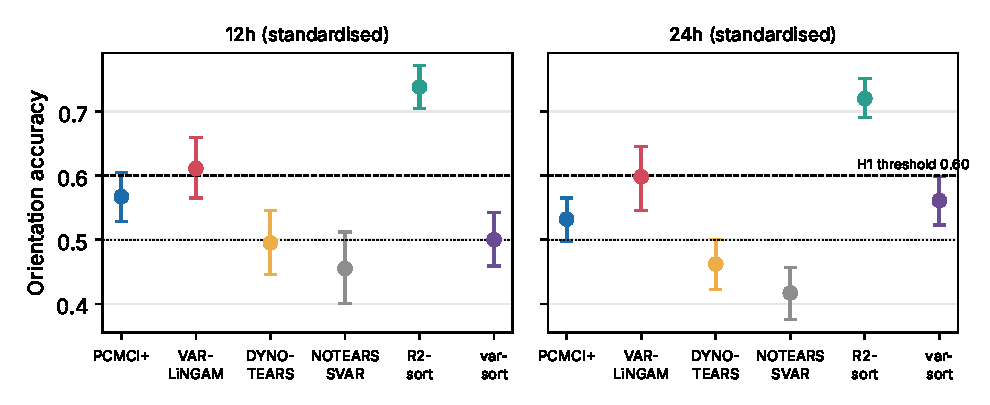
\includegraphics[width=0.95\linewidth]{generated/fig_orient}
\caption{Orientation accuracy on contemporaneous edges with 95\% bootstrap CIs. Dotted: chance; dashed: pre-registered 0.60. The mechanism-free R$^2$-sortnregress control is above all methods.}\label{fig:orient}
\end{figure}

\paragraph{H1 failed.}
The pre-registered H1 required, at both 12\,h and 24\,h, at least one contemporaneous-capable method (PCMCI+, VAR-LiNGAM, DYNOTEARS) with accuracy $\ge0.60$, a CI lower bound above 0.5, a mean paired AUROC gain over VAR of at least 0.03 and Holm $p<0.05$. At 12\,h only VAR-LiNGAM meets all conditions (0.611, CI [0.565, 0.660], AUROC gain +0.066, Holm $p=7.7\times10^{-6}$). At \textbf{24\,h no method meets them}: VAR-LiNGAM has accuracy 0.598 (just below 0.60; lower bound 0.546) with AUROC gain +0.083, PCMCI+ has 0.532 [0.498, 0.565] and DYNOTEARS 0.462 [0.423, 0.500]. H1 therefore fails. The two pre-registered negative criteria are also not met (VAR-LiNGAM is clearly above 0.5, and VAR has lower AUROC than every capable method), so the pre-registered overall verdict is \emph{ambiguous}. Including the NOTEARS-SVAR reference does not change this.

\paragraph{Orientation is weak and, for two methods, below chance.}
Besides VAR-LiNGAM, PCMCI+ is slightly above chance (0.53--0.57) and DYNOTEARS and the NOTEARS reference are at or below 0.5 on standardised data. The label-rule sensitivity does not change the picture (24\,h: VAR-LiNGAM 0.575 to 0.589 under the $\Delta/4$ and $\Delta$ rules, PCMCI+ 0.514 to 0.553). The $p=2$ run does not change the conclusions either, although VAR-LiNGAM falls to 0.504 at 24\,h and 0.583 at 12\,h. DYNOTEARS has a Gaussian least-squares objective with no non-Gaussianity step; on a synthetic check it reversed contemporaneous orientation on standardised data. Its poor orientation may therefore partly reflect the objective and partly our implementation, which we could not separate.

\paragraph{AUROC gains reflect skeleton detection.}
Contemporaneous-capable methods beat lag-only VAR in directed AUROC at every resolution (Table~\ref{tab:paired}), with Holm $p<0.05$ in all cases except VAR-LiNGAM at 6\,h. But the symmetric $|$correlation$|$ score, which orients nothing, has AUROC 0.684 at 24\,h (Figure~\ref{fig:auroc}), above VAR-LiNGAM (0.614) and DYNOTEARS (0.648) and level with PCMCI+ (0.689); at 12\,h it is 0.687 against 0.704 (PCMCI+) and 0.690 (DYNOTEARS). We did not run paired tests against correlation, so we only say the differences are small compared with the gaps to VAR. Lag-only VAR, whose lag-1 coefficients carry little same-step information at 24\,h, is simply a poor skeleton detector (0.531). Directed AUROC mixes detection and orientation; with orientation near chance the gain is mainly detection.

\begin{table}[t]\centering\small
\begin{tabular}{@{}llccc@{}}
\toprule
Res. & Method & $\Delta$AUROC vs VAR & raw $p$ & Holm $p$ (9) \\
\midrule
6h & PCMCI+ & +0.106 & 1.2e-09 & 5.9e-09 \\
6h & VAR-LiNGAM & +0.016 & 0.22 & 0.22 \\
6h & DYNOTEARS (own) & +0.112 & 4.5e-10 & 2.7e-09 \\
12h & PCMCI+ & +0.136 & 1.4e-10 & 9.8e-10 \\
12h & VAR-LiNGAM & +0.066 & 3.9e-06 & 7.7e-06 \\
12h & DYNOTEARS (own) & +0.123 & 7.7e-11 & 6.2e-10 \\
24h & PCMCI+ & +0.158 & 1.6e-13 & 1.5e-12 \\
24h & VAR-LiNGAM & +0.083 & 1.7e-06 & 5e-06 \\
24h & DYNOTEARS (own) & +0.117 & 1.3e-09 & 5.9e-09 \\
\bottomrule
\end{tabular}

\caption{Mean paired directed-AUROC difference to lag-only VAR; paired Wilcoxon, Holm over the 9 verdict-method pairs.}\label{tab:paired}
\end{table}

\begin{figure}[t]\centering
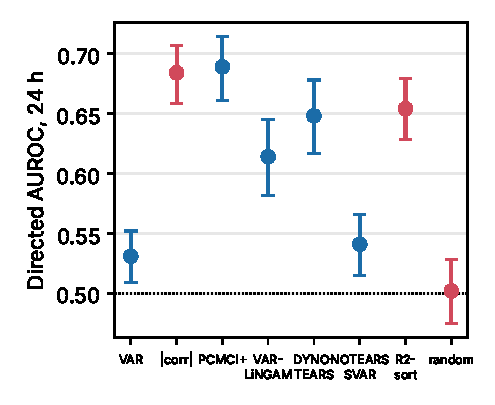
\includegraphics[width=0.5\linewidth]{generated/fig_auroc}
\caption{Directed AUROC at 24\,h with 95\% CIs. Red marks scores that use no contemporaneous causal modelling (correlation, R$^2$-sortnregress, random).}\label{fig:auroc}
\end{figure}

\paragraph{Controls: scale and explained variance.}
Table~\ref{tab:raw} contrasts raw and standardised data. R$^2$-sortnregress orients 0.738 (12\,h) and 0.720 (24\,h) of contemporaneous edges, better than every method; its directed AUROC (0.654 at 24\,h) also exceeds that of VAR-LiNGAM (0.614) and lag-only VAR (0.531). The plausible mechanism is that a downstream station is better explained by the others (it integrates upstream flows). On raw scale, var-sortnregress reaches 0.938 at 24\,h and the NOTEARS reference 0.865, while VAR-LiNGAM (0.740) and DYNOTEARS (0.765) gain 14 and 30 points over their standardised accuracy. PCMCI+ is identical on both scales (its tests are on partial correlations). Raw-scale orientation, and to a lesser extent explained-variance orientation, is thus available without any model of the mechanism. We did not retune DYNOTEARS or NOTEARS-SVAR $\lambda$ for raw scale.

\begin{table}[t]\centering\small
\begin{tabular}{@{}llcc@{}}
\toprule
Res. & Method & Acc. raw [95\% CI] & Acc. standardised \\
\midrule
12h & PCMCI+ & 0.567 [0.532, 0.603] & 0.567 \\
12h & VAR-LiNGAM & 0.755 [0.704, 0.803] & 0.611 \\
12h & DYNOTEARS (own) & 0.750 [0.699, 0.797] & 0.495 \\
12h & var-sortnregress & 0.941 [0.910, 0.967] & 0.500 \\
12h & R$^2$-sortnregress & 0.738 [0.704, 0.768] & 0.738 \\
\midrule
24h & PCMCI+ & 0.532 [0.502, 0.566] & 0.532 \\
24h & VAR-LiNGAM & 0.740 [0.697, 0.787] & 0.598 \\
24h & DYNOTEARS (own) & 0.765 [0.717, 0.809] & 0.462 \\
24h & var-sortnregress & 0.938 [0.912, 0.960] & 0.561 \\
24h & R$^2$-sortnregress & 0.720 [0.689, 0.750] & 0.720 \\
\bottomrule
\end{tabular}

\caption{Orientation accuracy on contemporaneous edges, raw versus standardised data.}\label{tab:raw}
\end{table}

\paragraph{Sibling residual correlation.}
To probe hidden shared drivers such as rain, we compute the mean correlation of VAR(1) residuals between stations that are both upstream parents of the same downstream station (siblings), between true-edge endpoints, and between all other pairs in the subgraph (Table~\ref{tab:sib}). At 24\,h siblings (0.508) correlate as strongly as other pairs (0.513) and less than adjacent stations (0.648). Contemporaneous dependence is large but not specific to river edges, so shared regional forcing contributes substantially to what a contemporaneous method sees. We have not separated forcing from direct propagation.

\begin{table}[t]\centering\small
\begin{tabular}{@{}lccc@{}}
\toprule
Res. & Siblings & Adjacent (true edge) & Other pairs \\
\midrule
6h & 0.320 & 0.413 & 0.303 \\
12h & 0.402 & 0.538 & 0.398 \\
24h & 0.508 & 0.648 & 0.513 \\
\bottomrule
\end{tabular}

\caption{Mean VAR(1) residual correlation (standardised, all 120 subgraphs).}\label{tab:sib}
\end{table}

\section{Pre-registration and deviations}
The plan (research/ts/02\_plan\_stage0.md, commit 3cd4581) and the gates were committed before any method ran; the hyperparameters were fixed on validation seeds before the test run. Deviations and operationalisations:
\begin{enumerate}
\item \textbf{Subgraph windows.} The plan's rule (drop a subgraph if any station keeps a gap after interpolating gaps of at most 2 steps) leaves no $d{=}10$ East German subgraph (only 92 of 666 East German stations are gap-free at all resolutions; the largest connected component among them has 6 nodes). We instead require a contiguous common window of at least 365 days per subgraph. This was decided before any label, gate or method result existed, but it selects well-measured stations.
\item \textbf{Aggregation rule.} Steps with fewer than 50\% of 15-minute values are set missing; the plan did not state this.
\item \textbf{DYNOTEARS $\lambda$ grid.} The best value ($0.1$) was at the edge of the original grid $\{0.001, 0.01, 0.1\}$; the grid was extended with $\{0.3, 1.0\}$ after the first validation run. 0.1 remained best. Selection used validation seeds only.
\item \textbf{NOTEARS-SVAR.} It is the plan's reference method and is excluded from the verdicts, with verdicts also shown with it included (no change).
\item \textbf{G1 and G3.} G1 passes pooled but not in East Germany (0.624). The G3 R$^2$ control reaches 0.72--0.74, below the 0.8 flag but far above 0.5; the flag did not trip, and we interpret the result more strictly than the rule.
\item \textbf{Operational decision rules} (verdict methods, Holm family, accuracy as a pooled-edge ratio) were written down before the test run in the gates file.
\end{enumerate}
The reading of the results in the abstract (skeleton detection, scale and explained-variance leakage, shared forcing) is post hoc and not pre-registered.

\section{Related work}
CausalRivers \citep{stein2025causalrivers} introduced the data and benchmarked lagged-structure methods over several resolutions, lags and normalisations, reporting the best hyperparameter combination per method. Its naive baselines include a magnitude-based orientation that is already competitive, which agrees with our scale-leakage finding; we did not find contemporaneous edges scored separately there. PCMCI \citep{runge2019pcmci} and PCMCI+ \citep{runge2020pcmciplus} handle lagged and contemporaneous links via conditional independence testing, VAR-LiNGAM \citep{hyvarinen2010svar} identifies contemporaneous direction from non-Gaussian noise, and DYNOTEARS \citep{pamfil2020dynotears} estimates contemporaneous and lagged matrices jointly under a continuous acyclicity constraint. Our checks are specific to this aggregated protocol and we do not survey other benchmarks here.

\section{Limitations}
\begin{itemize}
\item \textbf{One dataset cut.} Windows within 2019--2023 of 377--1826 days, drawn toward well-measured stations (deviation 1); results may not transfer to other windows or rivers.
\item \textbf{Linear methods only.} Nonlinear and neural methods may behave differently.
\item \textbf{Own DYNOTEARS implementation.} Checked only on one synthetic example; its below-chance orientation may partly be an implementation or objective artefact.
\item \textbf{Static travel time.} $\tauE$ is one estimate per edge, whereas true travel time varies with discharge; labels near the $\Delta/2$ boundary are noisy. G1 is weakest in East Germany.
\item \textbf{Overlapping sections.} The 100 test subgraphs contain overlapping river sections, so the cluster bootstrap over subgraphs is probably somewhat optimistic; and edges that occur in several subgraphs are counted per occurrence.
\item \textbf{Single dataset.} Without a second benchmark, we cannot say whether the leakage pattern is specific to rivers (discharge accumulates downstream) or common to aggregated real data.
\item \textbf{Hidden confounding.} We diagnose shared forcing via sibling residuals but do not model it.
\end{itemize}

\section{Conclusion}
Aggregating CausalRivers does create contemporaneous edges with a known direction, and the physics orientation is mostly supported by 15-minute data (G1 0.797 pooled, 0.624 in East Germany). As a test of contemporaneous modelling, the benchmark is weak: H1 fails (VAR-LiNGAM at 12\,h only), a control without any causal mechanism orients better than all methods, magnitude orients almost perfectly on raw scale, and shared forcing is as strong between unrelated stations as between siblings. Users of this protocol should report scale-only and explained-variance controls and a symmetric correlation baseline next to any contemporaneous method, and should not read AUROC gains over lag-only VAR as evidence of contemporaneous modelling.

\paragraph{Reproducibility.}
Code and result files are in research/ts/stage0 of the repository; tables and figures in this note are generated by research/ts/note/make\_assets.py from those result files.

\bibliographystyle{plainnat}
\bibliography{references}
\end{document}
